\documentclass[12pt]{article}

\usepackage{hyperref}
\usepackage{graphicx}

\begin{document}
\title{Activity III: Stellar Spectra}
\maketitle

\graphicspath{ {./images/} }

\section{Introduction and Objective}

In lecture we discussed stellar spectra, particularly in regards to the classification of stars. We have learned that there are three types of spectra; these
are continuous, emission, and absorption spectra. Continuous spectra are produced by objects emitting electromagnetic radiation (ER) along a continuum
with respect to wavelength (or frequency). Emission spectra are created by the
emission of ER at specific wavelengths. Absorption spectra, which are especially interesting to us, are formed by the absorption of specific wavelengths of light from a body emitting ER continuously. Stars’ spectra are of the absorption type.\newline
Stellar spectra are important in astronomy because they constitute an amalgam
of, by analogy, chemical fingerprints. Each element will absorb a specific set of wavelengths of light, determined via experiment. By comparing the spectrum of a star to elemental spectra, one can determine the chemical composition of the star–or, at least of the atmosphere of the star. Additionally, stellar spectra are integral to the classification system of stars that was introduced in lecture; namely, that stars are categorized according to decreasing surface temperature as one of the following: O, B, A, F, G, K, M, L, and T. The surface temperature of a star determines the state of the elements and the types of molecules (if any) that are present at the surface, and thus determines the spectrum. Let us present a succinct review of the Bohr model of the atom, which explains the physics of atoms that is pertinent to spectra.


\subsection{The Bohr Model of the Atom}

The idiosyncratic nature of quantum mechanics is illustrated by the discrete
nature of absorption (and emission) spectra, and allows astronomers to identify elements in stars’ atmospheres. In particular, the Bohr model, which is a
somewhat-antiquated atomic model proposed by Danish physicist Niels Bohr in
1913, asserts that electrons orbit around nuclei in discrete and circular orbits.
Unlike a macroscopic object such as the Earth, an electron must choose between one of a finite number of orbitals, each associated with a specific amount

% FIGURE 1 GOES HERE

\begin{center}
    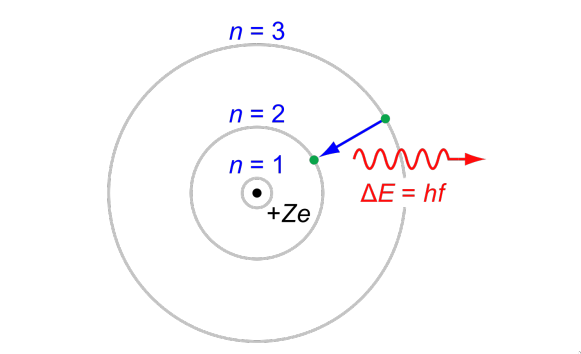
\includegraphics[scale=0.7]{fig1}
\end{center}

Figure 1: This figure illustrates the Bohr model [1] of the atom. \newline\newline
The orbits are discrete, and electrons must absorb a specific amount of energy in order to jump to an outer orbital. Correspondingly, an electron that jumps from an outer orbital to an inner one must emit light of a particular energy. In the figure, for example, an electron is seen falling from the first excited state to the ground state, emitting a photon as a result. To bring the electron back to the first excited state from the ground state, a photon of the same energy must be absorbed by the electron.\newline\newline 

of energy. If one were so inclined, one could slowly and incrementally nudge the Earth closer to, or farther from, the Sun. One cannot nudge an electron, however. To move it, one must impart to the electron a specific amount of energy equal to the difference between the orbital energy to which the electron will move, minus the orbital energy in which the electron initially resides. Therefore, in order for an electron to move to a higher energy level, it must absorb a specific amount of energy; this corresponds to a particular wavelength of light, since the energy of light is related to its wavelength. This explains absorption lines–from a continuous emission of a star, discrete wavelengths of light are absorbed by the atoms present in the star’s atmosphere. For further explanation, see [2, 3].

\subsection{Classifying Stellar Spectra}

Now let us discuss how to classify stars via their spectra. To do this, we must
determine the chemical compositions of stars’ atmospheres using stellar spectra. We study the spectrum of the star of interest, and match each absorption line to those of the elements and molecules that we have studied on Earth. In Figure 2, we list four spectra of unknown types, each from a different star. In Table 1, we list absorption wavelengths for some elements. See [4] for a more complete list.

Table 1: The below table lists select elements and some of their corresponding
absorption lines [4,5]. $H-\alpha$ through $H-\epsilon$ represent some transitions of the
Balmer series of the Hydrogen atom [5,6].

\begin{center}
\begin{tabular}{c | c}
atom & wavelength (nm) \\
\hline
\hline
H-$\alpha$ &  656.3 \\
H-$\beta$ & 486.1 \\
H-$\gamma$ & 434.1 \\
H-$\delta$ & 410.2 \\
H-$\epsilon$ & 397.0 \\
He & 587.6\\
He+  & 468.5\\
Ca+  & 393.4\\
Ca & 422.7\\
Ti & 396.5 \\
Si+  & 413.1\\
Fe & 404.6\\
Fe+ & 275.6\\
\hline
\end{tabular}
\end{center}


As we learned in class, the stellar classifications O-M indicate a decreasing
surface temperature scale–viz., it is the surface temperature of a star which
determines the absorbed wavelengths. In O type stars, extreme (> 2.5 × 104 K)
temperatures ionize much of the hydrogen (H). Thus, there is little H available to
absorb ER and the corresponding H spectral lines are weak. There are, however,
often strong ionized helium (He+) lines. In B stars, where surface temperatures
are considerably lower, neutral helium (He) exists in appreciable amounts and
hence these stars often exhibit strong neutral He lines. In B, A, and F type
stars, neutral H exists in abundance and these stars have the strongest H lines,
although A type stars yield the strongest H lines of the aforementioned types. In
particular, these stars produce strong Balmer lines, corresponding to the Balmer
series of H. These are lines associated with the transition of an electron to or
from the second energy level. See [6] for a review. The lower-temperature stars,
such as the M type, emit ER of generally insufficient energy to be absorbed by
H, and hence said lines are very weak in those stars.
Since metals are generally easier to ionize than nonmetals [7], ionized metals
begin to appear in A type stars and are very prevalent in F type stars. These
metals include ionized calcium (Ca+) and iron (Fe+), among others. Our Sun, a
G type star, creates neutral and ionized metal lines. Contrarily, in K and lower

% FIGURE 2a goes here

\begin{center}
    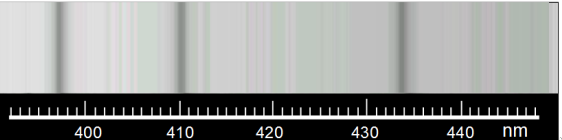
\includegraphics[scale=0.5]{fig2a}
\end{center}

\centerline{(a) The above figure is 2a.}

% FIGURE 2b goes here

\begin{center}
    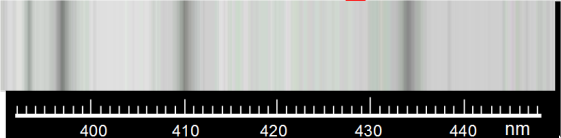
\includegraphics[scale=0.5]{fig2b}
\end{center}

\centerline{(b) The above figure is 2b.}

% FIGURE 2c goes here

\begin{center}
    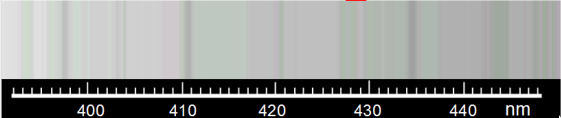
\includegraphics[scale=0.5]{fig2c}
\end{center}

\centerline{(c) The above figure is 2c.}

% FIGURE 2d goes here
\begin{center}
    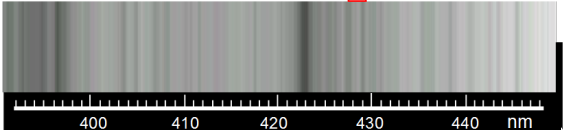
\includegraphics[scale=0.5]{fig2d}
\end{center}
\centerline{(d) The above figure is 2d.}

Figure 2: Figures 2a-2d depict four spectra of unknown types.\newline

type stars, only neutral metals typically appear–particularly in M type stars. K type stars can present Ca+ lines, however. In the coolest stars, molecules such as TiO can even appear. See [7,8] for further discussion.

\section{Experiment}

\subsection{Directions}

Read this activity carefully, and then study the spectra in Figure 2. Using the
resources present in this lab, in conjunction with your textbook and additional
web resources of your choosing, determine the spectral class associated with
each spectrum. Support your arguments with reasoning. Ensure that you only
quote scientific and professional sources.

\begin{enumerate}
        \item (2a) Elements that are present in the spectrum:
            \begin{enumerate}
                \item $H-\epsilon$
                \item $H-\delta$
                \item $H-\gamma$
            \end{enumerate}
            There is a lot of Hydrogen in this spectrum. Which means it must be a hot star with prominent hydrogen lines.\newline
            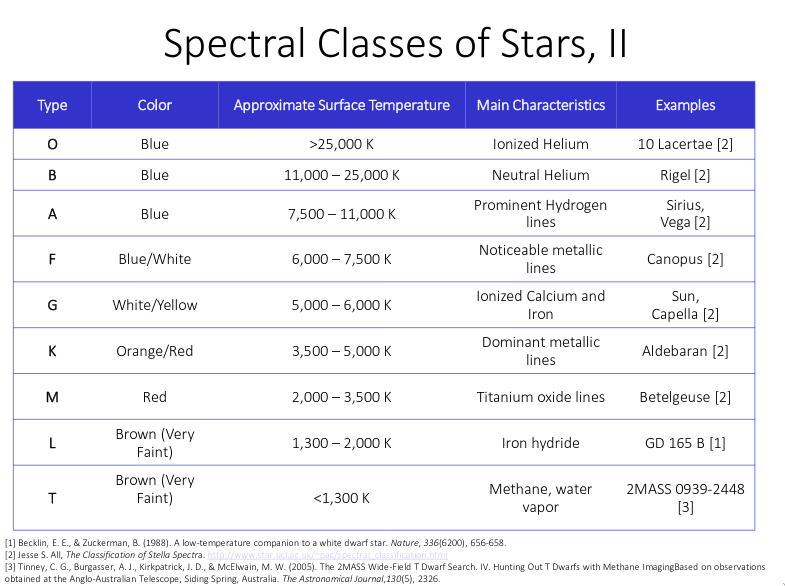
\includegraphics[scale=0.5]{spectral_table}
            Using the table provided in the lecture, I believe this star is an A type star.
        \item (2b) Elements that are present in the spectrum:
            \begin{enumerate}
                \item $H-\epsilon$
                \item $H-\delta$
                \item $H-\gamma$
                \item $Ca+$
            \end{enumerate}
            This spectrum seems to have very similar absorption lines to spectrum 2a except for one. There is ionized Calcium present in the spectrum. So far, it seems to be an A type star.\newline\newline
            As stated in section 1.2 "Classifying Stellar Spectra","A type stars and are very prevalent in F type stars. These metals include ionized calcium (Ca+) and iron (Fe+), among others". Here, there is ionized calcium and is therefore an A type star.

        \item (2c) Elements present in this spectrum:
            \begin{enumerate}
                \item $H-\gamma$
                \item $H-\epsilon$
                \item $H-\delta$
            \end{enumerate}
\end{enumerate}


\section{Conclusion}

Explain your conclusions in clear, complete sentences. Present your argument
for each case, supported with sufficient references and reasoning. You may type
or write your conclusions, but in either case they must be legible, clear, cogent,
and complete.


\section{References}
\begin{thebibliography}{8}
\bibitem{} JabberWok, \emph{The Rutherford-Bohr model of the hydrogen atom}, 2007, \href{https://commons.wikimedia.org/w/index.php?curid=2639910}{link}. Accessed: September 2016.
\bibitem{}Smith, Brian J., \emph{Chapter 4: The Bohr Model of the Atom}, \href{https://users.physics.ox.ac.uk/~smithb/website/coursenotes/qi/BohrModel.pdf}{link}. Accessed:
September 2016.
\bibitem{The Bohr Atom} De Leon, N., \emph{The Bohr Atom}, \href{http://www.iun.edu/~cpanhd/C101webnotes/modern-atomic-theory/Bohr-model.html}{link}. Accessed: September 2016.
\bibitem{} National Institute of Standards and Technology, \emph{Basic Atomic Spectroscopic Data}, \href{http://physics.nist.gov/PhysRefData/Handbook/atomic_number.htm}{link}. Accessed: September 2016.
\bibitem {} \emph{Measured Hydorgen Spectrum}, \href{http://hyperphysics.phy-astr.gsu.edu/hbase/tables/hydspec.html}{link}. Accessed: September 2016.
\bibitem{} Swinburne University of Technology, \emph{Balmer Series}, \href{http://astronomy.swin.edu.au/cosmos/B/Balmer+series}{link}. Accessed: September 2016.
\bibitem{} National Optical Astronomy Observatory, \emph{Stellar Spectroscopy}: The Message of Starlight, \href{https://www.noao.edu/education/astrobits/files/Stellar-Spectroscopy-Abits.pdf}{link}. Accessed: September 2016.
\bibitem{} \emph{Stellar Spectral Types}, \href{http://hyperphysics.phy-astr.gsu.edu/hbase/starlog/staspe.html}{link}. Accessed: September 2016.
\end{thebibliography}
————————————————

\end{document}
